%% ===================================================================
%% PART III (b): Sections 14-17
%% ===================================================================

\section{The outer hull chain and modular record geometry}\label{sec:chain}

Throughout this section $(d,s)$ is nonspecial and
\[
  Q=(d+u,\ d+v),\qquad 0\le u,v<d,\qquad(u,v)\ne(0,0).
\]
(The persistence result in Section~\ref{sec:persist} holds for all $Q\ge(d,d)$.) Put $H=H_Q$.

\subsection{Persistence of the lower-left hull}\label{sec:persist}

Let $c_0=A,\dots,c_n=B$ be the lower-left chain of $H_0$ and $v_i=(a_i,-b_i)=c_i-c_{i-1}$ its steps (Lemma~\ref{lem:chain0}); these are vectors of $\Gamma$. For each $i$ define
\[
  \varphi_i(z)=\frac{\cross(v_i,z)}{d}=\frac{a_iz_2+b_iz_1}{d},\qquad k_i=\varphi_i(c_{i-1})=\varphi_i(c_i).
\]
By Lemma~\ref{lem:det}, $\varphi_i(z)\in\Z$ for $z\in\Gamma$. The function $\varphi_i$ is increasing in both coordinates, $k_i\ge1$ (as $c_{i-1}\ne0$ lies in the quadrant), and the line $\varphi_i=k_i$ contains the $i$-th edge of the chain; $H_0$ lies in $\{\varphi_i\ge k_i\}$.

\begin{proposition}[Persistence]\label{prop:persist}
For every $Q\ge(d,d)$, every $q\in\Gamma\cap\R_{\ge0}^2\setminus\{0\}$ and every $i$, $\varphi_i(q)\ge k_i$. Consequently $H_Q\subseteq\{\varphi_i\ge k_i\}$ for all $i$, the lower-left chain of $H_0$ lies on $\partial H_Q$, and
\begin{equation}\label{eq:persist}
  H_Q\cap[0,d]^2=H_0.
\end{equation}
\end{proposition}
\begin{proof}
Let $q\in\Gamma$ be nonzero with $q\ge0$. While $q_1>d$ replace $q$ by $q-(d,0)$, and while $q_2>d$ by $q-(0,d)$. Each replacement stays in $\Gamma$ and in the quadrant, keeps $q\ne0$ (the coordinate being reduced stays positive), and strictly decreases every $\varphi_i$, by $a_id/d=a_i>0$ or $b_i>0$ respectively. The process ends at a nonzero point $q^*\in\Gamma\cap[0,d]^2$, that is $q^*\in F_{Q_0}\subseteq H_0$, so $\varphi_i(q)\ge\varphi_i(q^*)\ge k_i$. Thus $F_Q\subseteq\{\varphi_i\ge k_i\}$, and so is the convex hull $H_Q$.

Since the chain points are in $H_Q$ and satisfy $\varphi_i=k_i$ on the $i$-th edge, the edge lies on the supporting line of $H_Q$, hence in $\partial H_Q$. For \eqref{eq:persist}: $H_0\subseteq H_Q\cap[0,d]^2$ is clear. Conversely, the convex polygon $H_0$ is the intersection of the half-planes bounded by its edges, i.e. $H_0=\{x\le d\}\cap\{y\le d\}\cap\bigcap_i\{\varphi_i\ge k_i\}$ (the sides $AC_0$, $C_0B$ and the chain edges), and $H_Q\cap[0,d]^2$ satisfies all these inequalities.
\end{proof}

\begin{remark}
The same argument shows that every nonzero lattice point of the closed quadrant lies on the upper-right side of each supporting line of the chain; the chain is therefore part of the boundary of the convex hull of $\Gamma\cap\R_{\ge0}^2\setminus\{0\}$ (the Klein sail), as claimed in the remark after Theorem~\ref{thm:exceptional}.
\end{remark}

\subsection{\texorpdfstring{The outer chain $\Omega$}{The outer chain Omega}}

By Proposition~\ref{prop:persist}, $\partial H$ is the union of the lower-left chain from $A$ to $B$ and a second arc, from $B$ counterclockwise to $A$, which we call the \emph{outer arc}. Let $\Omega$ be the list of \emph{all} lattice points of $\Gamma$ on the outer arc in order from $B$ to $A$, including collinear ones and the end points $B$ and $A$. Consecutive points of $\Omega$ differ by Graver vectors (Lemma~\ref{lem:reflection}).

Label each $w\in\Omega$:
\[
  \begin{array}{ll}
  R:\ w_1\ge d,\ w_2<d; & C:\ w_1\ge d,\ w_2\ge d;\\
  T:\ w_1<d,\ w_2\ge d; & N:\ w_1<d,\ w_2<d.
  \end{array}
\]
Then $B$ has class $R$ and $A$ has class $T$.

\begin{figure}[ht]
\centering
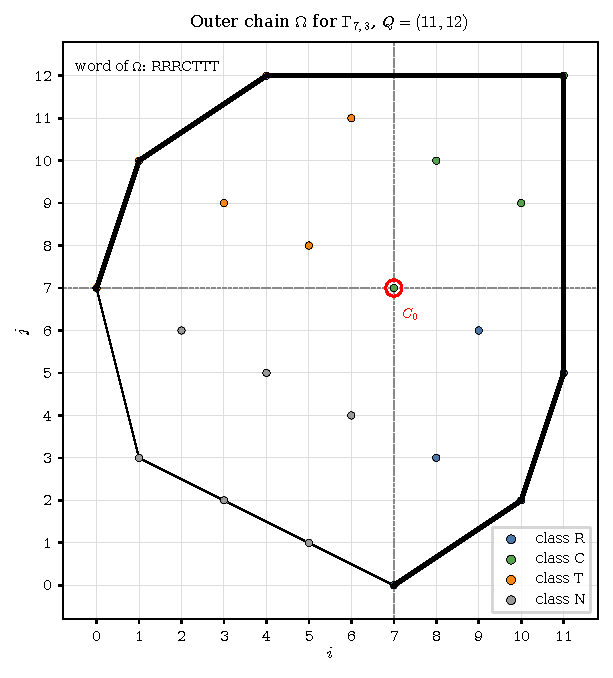
\includegraphics[width=.65\textwidth]{figures/fig08_chain.pdf}
\caption{The outer chain $\Omega$ (thick black) for $d=7$, $s=3$, $Q=(11,12)$, with points coloured by class ($R$ blue, $C$ green, $T$ orange); dashed lines are $x=d$ and $y=d$. Here $\Omega$ has the word $RRRCTTT$ and $C_0=(7,7)$ (red circle) lies in the \emph{interior} of $H_Q$, not on $\Omega$.}\label{fig:chain}
\par\smallskip\noindent\figdesc{A grid with the lattice points of $\Gamma_{7,3}$ in the box $[0,11]\times[0,12]$ coloured by class; the convex hull is outlined and its outer boundary from $B=(7,0)$ counterclockwise to $A=(0,7)$ is drawn thick. Two dashed lines mark $x=7$ and $y=7$ and the point $(7,7)$ is circled in red, inside the hull. The label above the picture spells the word of classes along the chain.}
\end{figure}

\begin{lemma}[Classification of the outer chain]\label{lem:omega}
\begin{enumerate}
\item $\Omega$ contains no point of class $N$.
\item The classes along $\Omega$ form a word in $R^*C^*T^*$.
\item No two consecutive points of $\Omega$ have classes $R$ and $T$ (in this order).
\item Consequently every edge $w\to w'$ of $\Omega$ has both abscissae $\ge d$ or both ordinates $\ge d$ (or both).
\end{enumerate}
\end{lemma}
\begin{proof}
(1) Let $w\in\Omega$ with $w_1,w_2<d$. Then $w\in H\cap[0,d]^2=H_0$ by \eqref{eq:persist}. A point of $H_0$ on $\partial H$ lies on $\partial H_0$ (an interior point of $H_0$ is an interior point of $H\supseteq H_0$). Since $w_1,w_2<d$ it does not lie on the sides $AC_0$ or $C_0B$ of $H_0$, hence lies on the lower-left chain. But the outer arc and the lower-left chain meet only at $A$ and $B$, which have classes $T$ and $R$. Contradiction.

(2) The point $B$ is the lowest point of $H$ (the only point of $\Gamma$ in the box on the $x$-axis other than the origin, because $d\mid x$ and $x<2d$), so counterclockwise from $B$ the outer arc first moves into the half-plane $x\ge d$ (to the right, or up along the side $x=d$ if $u=0$). The vertical line $x=d$ meets $H$ in a chord $[B,B']$, and the boundary of the convex polygon $H\cap\{x\ge d\}$ consists of this chord and one arc of $\partial H$ from $B$ to $B'$. Hence the points of $\Omega$ with $w_1\ge d$ are those on the arc from $B$ to $B'$, an initial segment of $\Omega$. In the same way, the point $A$ is the leftmost point of $H$ (the only point of $\Gamma$ in the box on the $y$-axis other than the origin when $v<d$ is $A$ itself, and $A$ has $x=0$), the line $y=d$ meets $H$ in a chord $[A,A']$, and the points of $\Omega$ with $w_2\ge d$ form the final segment of $\Omega$ from $A'$ to $A$. By (1) every point of $\Omega$ belongs to at least one of these two segments. Points in the initial segment but not the final one are of class $R$, in both of class $C$, in the final one only of class $T$. Since the initial segment is closed under taking predecessors and the final segment under taking successors, all $R$ points precede all $C$ points, which precede all $T$ points. So the word is in $R^*C^*T^*$.

(3) Let $w\in R$ and $w'\in T$ be consecutive. Put $\rho=w+w'-C_0$. Then
\[
  \rho_1=w_1+w'_1-d\in[w'_1,\,w_1),\qquad \rho_2=w_2+w'_2-d\in[w_2,\,w'_2),
\]
because $w'_1<d\le w_1$ and $w_2<d\le w'_2$; so $\rho\in\Gamma$ lies in the rectangle spanned by $w,w'$, inside the box. It is nonzero except possibly if $\rho=0$, which forces $w_1+w'_1=d$ and $w_2+w'_2=d$; with $w_1\ge d$ and $w'_2\ge d$ this gives $w=B$ and $w'=A$, which are never consecutive boundary lattice points of $H_Q$ (Lemma~\ref{lem:axis-pair} with $k=\ell=1$). So $\rho\in F_Q$, and so is $C_0$. Since $\rho+C_0=w+w'$, a supporting functional $\varphi$ of the side through $[w,w']$ satisfies $\varphi(\rho)+\varphi(C_0)=\varphi(w)+\varphi(w')=0$, hence $\varphi(C_0)=0$: the point $C_0$ lies on the supporting line. Its coordinates satisfy $w'_1<d=C_{0,1}\le w_1$ and $w_2<d=C_{0,2}\le w'_2$, so it lies in the rectangle spanned by $w,w'$ and, being on the line through them, on the segment $[w,w']$. It differs from both endpoints (as $w_2<d$ and $w'_1<d$). Thus $C_0$ is a lattice point strictly between consecutive boundary lattice points, a contradiction.

(4) Given (2) and (3), the possible consecutive class pairs are $RR,RC,CC,CT,TT$. In $RR,RC,CC$ both abscissae are $\ge d$; in $CC,CT,TT$ both ordinates are $\ge d$.
\end{proof}

\begin{remark}[The point $C_0$ need not lie on $\Omega$]\label{rem:D9}
Statement~(3) is proved by showing that $C_0$ cannot be a point strictly between two consecutive boundary lattice points of type $R,T$. It does \emph{not} assert that $C_0$ is a vertex of $\Omega$, nor that every $R$-to-$T$ passage runs through $C_0$. In fact $C_0$ can be an interior point of $H_Q$: for $d=5$, $s=2$, $Q=(8,8)$,
\[
  (5,5)=\tfrac19(5,0)+\tfrac13(0,5)+\tfrac59(8,6),
\]
with three points of $F_Q$ not collinear and all weights positive (check: $\frac19\cdot5+\frac59\cdot8=5$ and $\frac13\cdot5+\frac59\cdot6=5$). So $C_0\in\interior H_Q$. The older source text (GEO-I v012, MIXED\_CAP) said that $C_0$ is on a bridging edge of the outer chain; that statement is false and is not used here. This is correction D9 of Appendix~\ref{app:corrections}. In Figure~\ref{fig:chain} the same phenomenon is visible: $C_0$ is interior.
\end{remark}

\subsection{First and last step}

Let $u\ge1$. For $1\le i\le u$ put $r_i=si\bmod d\in\{1,\dots,d-1\}$ (nonzero since $0<i<d$ and $s$ is a unit). The $r_i$ are pairwise distinct (as $i\mapsto si$ is injective mod $d$). Let $y=\min_{1\le i\le u}r_i$, attained at the unique index $x$, and
\[
  M=(x,y).
\]
Since $r_1=s$, $y\le s$; and $x\le u$.

\begin{lemma}[Records]\label{lem:records}
\begin{enumerate}
\item $M\in\Gamma$ is Pareto-minimal; in particular $M$ is a Graver vector.
\item $r_i/i>y/x$ for $1\le i<x$, and $r_i/i\ge y/x$ for $x<i\le u$.
\item The first edge of $\Omega$ is $B\to B+M$; the point $B+M=(d+x,y)$ has class $R$.
\end{enumerate}
\end{lemma}
\begin{proof}
(1) $y\equiv sx$ so $M\in\Gamma$. Let $(i,j)\in\Gamma\cap[0,x]\times[0,y]$. If $i=0$ then $d\mid j\le y<d$, so $j=0$ and the point is the origin. If $1\le i\le x$ ($\le u$) then $j\equiv si$ with $0\le j<d$ gives $j=r_i\ge y$ by minimality of $y$, so $j=y$, $i=x$. Hence $\Gamma\cap[0,x]\times[0,y]=\{0,M\}$. The Graver property was shown after the definition of Pareto-minimality.

(2) For $i<x$: $r_i>y$ (as $x$ is the unique index of the minimum), so $r_i/i>y/x$. For $i>x$ suppose $r_i/i<y/x$ and, among such $i\le u$, take the smallest. Then $r_i\ge y$ and $i'=i-x\ge1$, $r_i-y\equiv si'$, $0\le r_i-y<d$ and $r_i-y\ne0$ (else $d\mid i'$ with $0<i'<d$). So $r_{i'}=r_i-y$ and
\[
  \frac{r_{i'}}{i'}=\frac{r_i-y}{i-x}<\frac yx
\]
(because $r_ix<yi$ implies $x(r_i-y)<y(i-x)$). If $i'>x$ this contradicts the minimality of $i$; if $i'=x$ it contradicts $r_x/x=y/x$; if $i'<x$ it contradicts $r_{i'}/i'>y/x$ from the first part. Hence $r_i/i\ge y/x$ for all $i\le u$.

(3) The points of $F_Q$ with abscissa $d+i$, $1\le i\le u$, have ordinates $\equiv si\pmod d$ and $\ge0$, hence $\ge r_i$; all points of $F_Q$ with abscissa $\le d$ lie above or on the line through $B$ of slope $y/x$ extended to the left (their ordinates are $\ge0$ while the line has negative ordinates there, and $C_0$ lies above it). The displacement from $B$ to $(d+i,j)$ has slope $j/i\ge r_i/i\ge y/x$ by (2). So the line through $B$ and $B+M$ supports $H$, and $B+M=(d+x,y)\in F_Q$ (as $x\le u$ and $y<d\le Q_2$). By Pareto-minimality no lattice point lies strictly between $B$ and $B+M$. Thus $B+M$ is the point following $B$ on the outer arc.
\end{proof}

(Equality in (2) can occur, for example at $i=2x$ if $2y<d$ and $2x\le u$; then $B+2M$ lies on the same supporting line, further from $B$ than $B+M$.)

If $u=0$ there are no points of $F_Q$ with abscissa $>d$; then $Q_1=d$ and the first edge of $\Omega$ runs up the side $x=d$ from $B$ to $C_0$.

\begin{lemma}[Last step]\label{lem:last}
Let $v\ge1$ and let $N=(N_1,N_2)$ be the transposed record: $N_1=\min_{1\le j\le v}(tj\bmod d)$, $N_2$ its unique index $j$. Then $N$ is Pareto-minimal, the point $A+N=(N_1,d+N_2)$ lies in $F_Q$ and has class $T$, and the last edge of $\Omega$ is $A+N\to A$.
\end{lemma}
\begin{proof}
Apply Lemma~\ref{lem:records} to the transposed instance $(d,t,(Q_2,Q_1))$ and transpose back (Proposition~\ref{prop:elem}(5)): the outer arc of the transposed hull is the reversal of the outer arc of $H$, with $B$ and $A$ interchanged.
\end{proof}

%% -------------------------------------------------------------------
\section{Explicit construction of the covering cell family}\label{sec:cellfamily}

Fix a nonspecial class and $Q=(d+u,d+v)$ with $0\le u,v<d$, $(u,v)\ne(0,0)$. Let $\Omega=(w^{(0)}=B,\ w^{(1)},\dots,w^{(\mu)}=A)$.

\begin{table}[ht]
\centering\small
\begin{tabular}{@{}p{3.2cm}p{7.2cm}p{4.2cm}@{}}
\toprule
Family & Cells & Role\\
\midrule
L-cells & $P(w;\,w'-w,\,(-d,0))$ for $\Omega$-edges $w\to w'$ with both abscissae $\ge d$, except the first edge & sweep the cap horizontally\\
D-cells & $P(w;\,w'-w,\,(0,-d))$ for $\Omega$-edges with both ordinates $\ge d$, except the last edge & sweep the cap vertically\\
bottom cell $\mathcal B$ ($u\ge1$) & $P(B-g;\,g,\,M)$ & covers the first-edge region $\Delta_B$\\
left cell $\mathcal A$ ($v\ge1$) & $P(A-h;\,h,\,N)$ & covers the last-edge region $\Delta_A$\\
\bottomrule
\end{tabular}
\caption{The cap family $\mathcal C_Q$ for $Q=(d+u,d+v)$.}\label{tab:capfamily}
\end{table}

\subsection{L-cells and D-cells}

\begin{lemma}[L-cells]\label{lem:L}
Let $w\to w'$ be an edge of $\Omega$ with $w_1,w'_1\ge d$ which is not the first edge ($w\ne B$). Then $P(w;\,w'-w,\,(-d,0))$ is an admissible parallelogram. Its corners are $w,\ w',\ w-(d,0),\ w'-(d,0)$.
\end{lemma}
\begin{proof}
$w'-w$ is Graver by Lemma~\ref{lem:reflection} and $(-d,0)$ is Graver. They are independent: a horizontal vector of $\Gamma$ is divisible by $d$ in its first coordinate, while $w_1,w'_1\in[d,d+u]$ and $u<d$ give $|w'_1-w_1|<d$; so $w'-w$ is horizontal only if it is zero, which it is not. The corners $w-(d,0)$ and $w'-(d,0)$ lie in $\Gamma$ and have abscissae $\ge0$ and ordinates equal to those of $w,w'$, so they lie in the box. They are nonzero: the corner $w-(d,0)$ is zero iff $w=B$, excluded, and $w'-(d,0)=0$ iff $w'=B$, impossible since $B$ is the first point of $\Omega$.
\end{proof}

\begin{lemma}[D-cells]\label{lem:D}
Let $w\to w'$ be an edge of $\Omega$ with $w_2,w'_2\ge d$ which is not the last edge ($w'\ne A$). Then $P(w;\,w'-w,\,(0,-d))$ is admissible.
\end{lemma}
\begin{proof}
The transposed statement of Lemma~\ref{lem:L}, using $v<d$.
\end{proof}

\subsection{The bottom cell and the left cell}

Let $u\ge1$ and $M=(x,y)$ be the record of Lemma~\ref{lem:records}. By Lemma~\ref{lem:arith} one of the two numbers
\[
  \cross\bigl((1,-a),M\bigr)=y+ax,\qquad \cross\bigl((c,-1),M\bigr)=x+cy
\]
is at least $xy$. Choose $g\in\{(1,-a),(c,-1)\}$ with $\cross(g,M)\ge xy$ (if both qualify, take the first). Both vectors are Graver by Lemma~\ref{lem:std-graver}. Define the \emph{bottom cell}
\[
  \mathcal B=P(B-g;\ g,\ M)=B+[0,1]M-[0,1]g.
\]

\begin{lemma}[Bottom cell]\label{lem:bottom}
$\mathcal B$ is admissible and contains the triangle $\Delta_B=\conv\bigl(B,\ B+M,\ (d,y)\bigr)$.
\end{lemma}
\begin{proof}
\emph{Corners.} For $g=(1,-a)$ the corners are $B-g=(d-1,a)$, $B$, $B-g+M=(d-1+x,\,a+y)$ and $B+M=(d+x,y)$. Since $x\le u$ and $y\le s$ we have $d-1+x\le Q_1$ and $a+y\le a+s=d\le Q_2$. For $g=(c,-1)$ they are $(t,1)$, $B$, $(t+x,\,1+y)$ and $B+M$, with $t+x\le d-1+u$ and $1+y\le s+1\le d$. All have positive coordinates, lie in $\Gamma$ (as $g,M\in\Gamma$ and $B\in\Gamma$) and so in $F_Q$. \emph{Independence.} $\cross(g,M)\ge xy>0$.

\emph{Containment.} Relative to $B$ we need $(0,y)=\alpha M-\beta g$ with $\alpha,\beta\in[0,1]$ (the vertices $B$ and $B+M$ of $\Delta_B$ are obviously in $\mathcal B$). Solving the two linear equations,
\[
  \beta=\frac{xy}{\cross(g,M)},\qquad\alpha=\frac{g_1\,y}{\cross(g,M)}.
\]
Here $0<\beta\le1$ by the choice of $g$, and $0<\alpha\le1$ because $\cross(g,M)=g_1y-g_2x=g_1y+|g_2|x\ge g_1y$. Hence $(d,y)\in\mathcal B$ and $\Delta_B\subseteq\mathcal B$ by convexity.
\end{proof}

For $v\ge1$ the \emph{left cell} $\mathcal A$ is defined by transposition: with the record $N=(N_1,N_2)$ of Lemma~\ref{lem:last}, choose $h\in\{(-1,a),(-c,1)\}$ with $\cross(N,h)\ge N_1N_2$ (the two values are $aN_1+N_2$ and $N_1+cN_2$, and one of them is $\ge N_1N_2$ by Lemma~\ref{lem:arith}, applied with $x=N_1$, $y=N_2$), and put
\[
  \mathcal A=P(A-h;\ h,\ N)=A+[0,1]N-[0,1]h.
\]
By transposition, $\mathcal A$ is admissible and contains $\Delta_A=\conv(A,\ A+N,\ (N_1,d))$.

\begin{figure}[ht]
\centering
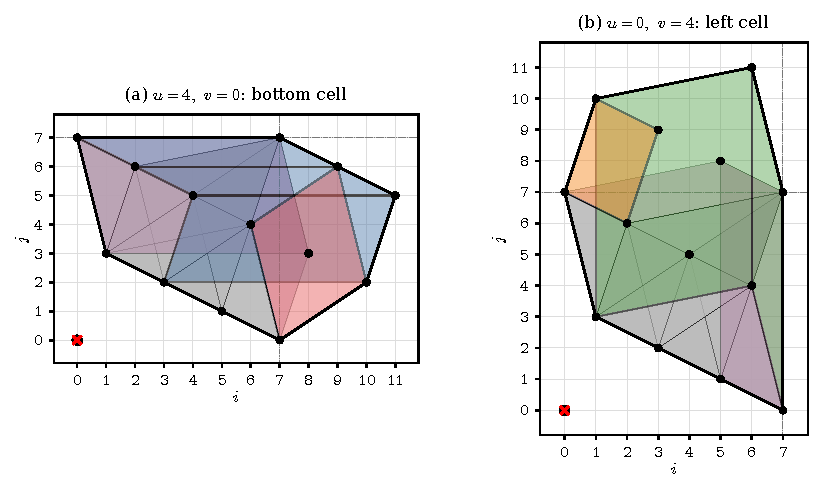
\includegraphics[width=\textwidth]{figures/fig10_endcells.pdf}
\caption{Bottom and left cells, $d=7$, $s=3$. (a) $Q=(11,7)$ ($u=4$, $v=0$): a bottom cell is needed for the first edge. (b) $Q=(7,11)$ ($u=0$, $v=4$): the transposed left cell. All other colours are as in Figure~\ref{fig:sweeps}.}\label{fig:endcells}
\par\smallskip\noindent\figdesc{Two panels. Left: a $11\times7$ box with the convex hull shaded by overlapping cells; a differently coloured parallelogram sits at the lower right corner, adjacent to $B$. Right: the transposed picture, a differently coloured parallelogram at the upper left, adjacent to $A$.}
\end{figure}

\begin{figure}[ht]
\centering
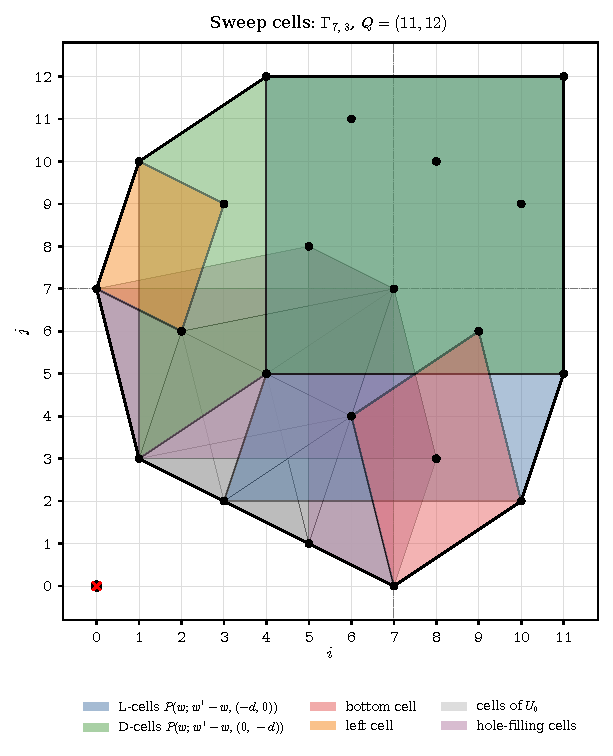
\includegraphics[width=.65\textwidth]{figures/fig09_sweeps.pdf}
\caption{The complete cell family for $d=7$, $s=3$, $Q=(11,12)$ ($u=4$, $v=5$): cells of $U_0$ (grey-green), hole-filling cells $R_1,R_2$ (and transposes), L-cells, D-cells, bottom and left cells. Together with $H_0\subseteq U_Q$ they cover $H_Q$.}\label{fig:sweeps}
\par\smallskip\noindent\figdesc{A $11\times12$ box with the convex hull of the lattice points of $\Gamma_{7,3}$ covered by overlapping coloured parallelograms; the legend below lists the cell families: L-cells, D-cells, bottom cell, left cell, cells of $U_0$, hole-filling cells.}
\end{figure}

%% -------------------------------------------------------------------
\section{Complete coverage of the nonexceptional cap}\label{sec:cap}

\begin{theorem}[Small-box cap coverage; GEO-I G12-T3--T7]\label{thm:cap}
Let $(d,s)$ be nonspecial and $Q=(d+u,d+v)$, $0\le u,v<d$, $(u,v)\ne(0,0)$. Then $H_Q\setminus H_0\subseteq\bigcup\mathcal C_Q$, where $\mathcal C_Q$ is the cap family of Table~\ref{tab:capfamily}. Consequently $U_Q=H_Q$.
\end{theorem}

\subsection{Proof}

\emph{Reduction to generic points.} Let $G$ be the finite set of all horizontal and all vertical lines passing through a lattice point of $\Gamma$ on $\partial H$ (all of them, not only the vertices of $H$), together with the lines $x=d$ and $y=d$. Call a point $z$ \emph{generic} if $z\in\interior H$ and $z\notin\bigcup G$. Generic points are dense in $H$, the union $\bigcup\mathcal C_Q\cup U_0$ is a finite union of closed sets, hence closed, and every point of $H_0$ is in $U_Q$ by Corollary~\ref{cor:old}. So it is enough to show that every generic $z\in H\setminus H_0$ lies in $\bigcup\mathcal C_Q$. By \eqref{eq:persist}, such a $z$ has $z_1>d$ or $z_2>d$. The condition ``generic'' (avoiding the horizontal and vertical lines through \emph{every} boundary lattice point) will be used to place exit points strictly between consecutive boundary lattice points; avoiding only the lines through the vertices of $H$ would not suffice, since the exit point could then be a non-vertex boundary lattice point.

By transposition (which commutes with the cap construction: it exchanges L-cells with D-cells, the bottom cell with the left cell, and the roles of $u,v$, and preserves genericity), the points with $z_1<d<z_2$ follow from the points with $z_2<d<z_1$. So there remain two cases: (1a) $z_1>d>z_2$ and (1b) $z_1>d$, $z_2>d$.

\emph{The horizontal exit point.} Let $z$ be generic with $z_1>d$ (so $u\ge1$). Let $p$ be the point at which the ray $z+\tau(1,0)$, $\tau\ge0$, leaves $H$; $p_1>z_1$ and $p_2=z_2$. Since $z_2$ differs from the ordinate of every boundary lattice point, $p$ is not a boundary lattice point, in particular not a vertex of $H$. Hence $p$ lies in the relative interior of a segment $[w,w']$ joining two \emph{consecutive} boundary lattice points of $H$. This segment is not horizontal, since otherwise $p_2=w_2$.

The point $p$ is the rightmost point of the horizontal slice of $H$ at the height $z_2$. We claim that $[w,w']$ is an edge of the outer chain $\Omega$ in its \emph{ascending part}, that is, the part of $\Omega$ from $B$ up to a highest point of $H$, along which the ordinate is nondecreasing. Indeed, the lowest point of $H$ is $B$ (the only lattice point of the box on the $x$-axis is $B$, since $d\mid x$), so counterclockwise from $B$ the ordinate increases up to the top of $H$ and then decreases; the right ends of the horizontal slices at heights between $0$ and the maximal ordinate lie on the ascending part, and the lower-left chain contains the left ends of its slices. Thus $[w,w']=$ an edge $w\to w'$ of $\Omega$ with $w_2\le w'_2$, and since the edge is not horizontal, $w_2<z_2<w'_2$. By Lemma~\ref{lem:omega}(4), since the edge contains the point $p$ with $p_1>d$, it is of type $RR$, $RC$, $CC$ or $CT$ (type $TT$ has all abscissae $<d$). The key distance estimate is
\begin{equation}\label{eq:dist}
  0<p_1-z_1<Q_1-d=u<d,
\end{equation}
since $p\in H\subseteq[0,Q_1]^2$-box and $z_1>d$.

\emph{Case 1a: $z_1>d>z_2$.} Then $p_2=z_2<d$, so the edge contains a point with ordinate $<d$; edges of type $CC$ and $CT$ have both endpoints with ordinate $\ge d$, hence all their points do. So the edge has type $RR$ or $RC$: both abscissae are $\ge d$.
\begin{itemize}
\item If $w\ne B$, the L-cell $P(w;w'-w,(-d,0))$ of Lemma~\ref{lem:L} is in $\mathcal C_Q$. Its horizontal slice at the height $z_2$ is $[p_1-d,\,p_1]$. By \eqref{eq:dist}, $p_1-d<z_1<p_1$, so $z$ lies in the slice, hence in the cell.
\item If $w=B$, the edge is the first edge $B\to B+M$ (Lemma~\ref{lem:records}), and $z_2\in(0,y)$. The slice of $\Delta_B$ at the height $z_2$ is $[d,\ d+xz_2/y]=[d,p_1]$, which contains $z$ since $d<z_1<p_1$. So $z\in\Delta_B\subseteq\mathcal B$ by Lemma~\ref{lem:bottom}.
\end{itemize}

\emph{Case 1b: $z_1>d$, $z_2>d$.} (Then $v\ge1$.) The edge contains the point $p$ with $p_2=z_2>d$. An $RR$ edge has both ordinates $<d$, so the type is $RC$, $CC$ or $CT$. The first edge $B\to B+M$ has both endpoints of ordinate $<d$ (type $RR$), so $w\ne B$.
\begin{itemize}
\item If the type is $RC$ or $CC$, both abscissae are $\ge d$, the L-cell of the edge is in $\mathcal C_Q$ (Lemma~\ref{lem:L}), and, exactly as in Case~1a using \eqref{eq:dist}, it contains $z$.
\item If the type is $CT$, so $w_1\ge d>w'_1$, both ordinates are $\ge d$. The edge is not the last edge of $\Omega$, which is $A+N\to A$ with starting point of class $T$ (Lemma~\ref{lem:last}), whereas $w$ has class $C$. So the D-cell $P(w;w'-w,(0,-d))$ of Lemma~\ref{lem:D} is in $\mathcal C_Q$. Along this edge, in the direction from $w$ to $w'$, the abscissa decreases (from $\ge d$ to $<d$) and the ordinate is nondecreasing, so the edge is the graph of a decreasing function over $[w'_1,w_1]$, and $H$ lies below and to the left of it (the edge is part of the ascending boundary, with outward normal in the open first quadrant). Since $w'_1<d<z_1<p_1\le w_1$, the vertical line through $z$ meets this edge at the point $q=(z_1,q_2)$ with $q_2\ge p_2=z_2$, and $q_2>z_2$ as $z_1<p_1$. The point $q$ is the top of the vertical slice of $H$ at the abscissa $z_1$, so $q_2\le Q_2=d+v$. Hence
\[
  0<q_2-z_2\le Q_2-z_2<Q_2-d=v<d.
\]
The vertical slice of the D-cell at the abscissa $z_1$ is $[q_2-d,\,q_2]$, which therefore contains $z_2$. So $z$ is in the D-cell.
\end{itemize}
If $v=0$ no generic point has $z_2>d$ and Case 1b is vacuous.

This covers all generic points of $H\setminus H_0$, and by closedness all of $H\setminus H_0$. Together with $H_0\subseteq U_Q$ (Corollary~\ref{cor:old}) we obtain $H_Q\subseteq U_Q$, and $U_Q\subseteq H_Q$ always. \qed

\subsection{Remarks on the proof}

\begin{remark}[Mixed enlargements]
The proof treats $(u,v)$ with $u,v\ge1$, $u\ge1=v-1$, and the one-sided cases $u=0$ or $v=0$ in the same framework. If $v=0$ the last edge of $\Omega$ is $C_0\to A$ (of type $CT$) and nothing above $y=d$ has to be covered; if $u=0$ there are no generic points with $z_1>d$, the first edge of $\Omega$ is $B\to C_0$, and Case~1a is vacuous, while the transposed cases cover the cap above $H_0$.
\end{remark}

\begin{remark}[No residual corner region]
An earlier version of the argument (the GEO-I v011 proof) covered all of the cap except a small polygonal region near $C_0$, a pentagon, which was then treated separately; that pentagon was found to be wrongly described and was corrected. In the present proof no such region arises: every generic point of $H\setminus H_0$ is placed in one of the cells by following a horizontal ray to the ascending right boundary and, if the edge reached crosses $x=d$, a vertical ray to the same edge. In particular the proof never needs to know where $C_0$ lies relative to $\Omega$ (Remark~\ref{rem:D9}).
\end{remark}

\begin{figure}[ht]
\centering
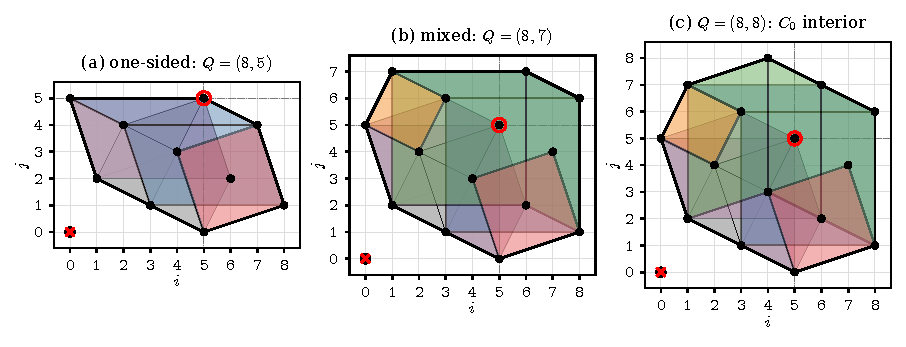
\includegraphics[width=\textwidth]{figures/fig11_cap.pdf}
\caption{Complete coverage for $d=5$, $s=2$: (a) one-sided enlargement $Q=(8,5)$, (b) mixed enlargement $Q=(8,7)$, (c) $Q=(8,8)$, where $C_0=(5,5)$ (red circle) is an interior point of $H_Q$ (correction D9). In each case the coloured cells cover the whole hull.}\label{fig:cap}
\par\smallskip\noindent\figdesc{Three panels with the hull of the lattice points of $\Gamma_{5,2}$ in boxes $8\times5$, $8\times7$, $8\times8$, each completely covered by overlapping coloured parallelograms; in the third panel a red circle marks $(5,5)$ inside the hull.}
\end{figure}

%% -------------------------------------------------------------------
\section{Main theorem: universal planar convex stabilization}\label{sec:main}

\begin{theorem}[Universal planar convex stabilization; GEO-I G12-T8]\label{thm:universal}
For every integer $d\ge2$, every unit $s$ modulo $d$ and every integer box $Q=(Q_1,Q_2)$ with $Q_1,Q_2\ge d$ and $Q\ne(d,d)$,
\[
  \boxed{\,U_{d,s,Q}=\conv\bigl(F_{d,s,Q}\bigr)\,}.
\]
\end{theorem}

\begin{proof}
The proof is a case distinction. The inclusion $U_Q\subseteq H_Q$ always holds (Proposition~\ref{prop:elem}), so only $H_Q\subseteq U_Q$ is to be shown.
\begin{center}
\small
\begin{tabular}{@{}p{5.4cm}p{4.2cm}p{4.8cm}@{}}
\toprule
Parameter regime & Argument & Dependencies\\
\midrule
$s\equiv\pm1$ (all $d\ge2$; this includes every unit for $d=2,3,4,6$) & Theorem~\ref{thm:L} & Lemma~\ref{lem:special-graver}\\
$\max(Q_1,Q_2)\ge2d$ & Theorem~\ref{thm:large} & Lemmas~\ref{lem:columns}, \ref{lem:reflection}\\
$d\ge5$ nonspecial, $Q=(d+u,d+v)$, $0\le u,v<d$ & Corollary~\ref{cor:old} + Theorem~\ref{thm:cap} & Sections~\ref{sec:exceptional}--\ref{sec:fill}, \ref{sec:pareto}--\ref{sec:cellfamily}\\
$Q=(d,d)$ & excluded; classified in Part~II & Theorem~\ref{thm:exceptional}, Propositions~\ref{prop:special-fan}, \ref{prop:special-plus}\\
\bottomrule
\end{tabular}
\end{center}
If $s\equiv\pm1$ apply Theorem~\ref{thm:L}. Otherwise $(d,s)$ is nonspecial, so $d\ge5$. If $\max(Q_1,Q_2)\ge2d$ apply Theorem~\ref{thm:large}. If $\max(Q_1,Q_2)<2d$ then $Q=(d+u,d+v)$ with $0\le u,v<d$ and $(u,v)\neq(0,0)$ since $Q\ne(d,d)$; then $H_0\subseteq U_Q$ by Corollary~\ref{cor:old} and $H_Q\setminus H_0\subseteq U_Q$ by Theorem~\ref{thm:cap}. These cases exhaust the hypotheses.
\end{proof}

\begin{corollary}[Convexity and contractibility]\label{cor:contractible}
Under the hypotheses of Theorem~\ref{thm:universal}, $U_{d,s,Q}$ is a compact convex polygon with vertices in $F_{d,s,Q}$. In particular it is contractible: $\beta_0=1$ and $\beta_k=0$ for $k\ge1$.
\end{corollary}

\begin{corollary}[Persistence of stabilization]\label{cor:persistence}
If $Q\ge(d,d)$, $Q\ne(d,d)$, then $U_{Q'}=H_{Q'}$ for all $Q'\ge Q$. In particular a nonexceptional box never reverts to a nonconvex union as it grows. Together with Theorem~\ref{thm:betti}, the first Betti number of $U_{d,s,Q}$ over all boxes $Q\ge(d,d)$ is $d$ (resp. $2$) at $Q=(d,d)$ for $s\equiv-1$ (resp. otherwise) and $0$ for every other box.
\end{corollary}

\begin{corollary}[Application to an actual planar occurrence fibre]\label{cor:actual}
In the arithmetic setting of Section~\ref{sec:planar}, let $x=a/b$ have two active prime coordinates and assume $d\ge2$,
\[
  q_i\ge o_i\quad(i=1,2),\qquad \bigl(\lfloor q_1/\lambda_1\rfloor,\lfloor q_2/\lambda_2\rfloor\bigr)\ne(d,d).
\]
Then the realized Graver-cell union of the occurrence fibre $F_x\subset\Lambda_b$ equals its convex hull and is contractible. The excluded case is the arithmetic plateau
\[
  o_1\le q_1\le o_1+\lambda_1-1,\qquad o_2\le q_2\le o_2+\lambda_2-1;
\]
there $\beta_1(U)=d$ if $s\equiv-1\pmod d$ and $\beta_1(U)=2$ otherwise.
\end{corollary}
\begin{proof}
By Corollary~\ref{cor:plateau} the hypotheses say $Q_i\ge d$ and $Q\ne(d,d)$ for the normalized box. By Proposition~\ref{prop:transfer} the realized union of the actual fibre is $L(U_{d,s,Q})$, so Theorem~\ref{thm:universal} and Corollary~\ref{cor:contractible} apply. On the plateau Theorem~\ref{thm:betti} applies.
\end{proof}

\begin{remark}[What the theorem does not say]
The theorem does not assert that the admissible cells form a face-to-face subdivision of $H_Q$, or that the abstract complex $K_{\mathrm{abs}}(Q)$ is contractible; it asserts that the \emph{set} $U_Q$ equals the hull. It says nothing for $d=1$, for boxes with a side below $d$, for fibres with three or more active primes, or about the relation between the geometry of different values.
\end{remark}
